\def\finalpaper{1} % use 1 for final and 0 for anonymous submission

\def\replaceTAAL{1}

\documentclass[conference]{IEEEtran}
\usepackage{pgf-pie}  
\usepackage{dblfloatfix}
% to be able to draw some self-contained figs
\usepackage{balance}
\usepackage{tikz}
\usepackage{amsmath}
\usepackage{amsfonts}
\usepackage[ruled,linesnumbered]{algorithm2e}
\setlength{\algomargin}{2em}
% inlined bib file
\usepackage{filecontents}
\usepackage{cuted,adjustbox}
\usepackage{multirow,multicol}
\usepackage{booktabs,colortbl}
\usepackage{pgfplots} 
\usetikzlibrary{patterns}
\usepackage[labelformat=simple]{subcaption}
\renewcommand\thesubfigure{(\alph{subfigure})}
\usepackage{rotating}
%\usepackage{titling}
%% Code styles
\usepackage{xcolor}
\definecolor{rwth_blue}{RGB}{0,84,159}
\definecolor{rwth_green}{RGB}{87,171,39}
\definecolor{rwth_red}{RGB}{204,7,30}
\usepackage{circledsteps}
\usepackage{xspace}
\usepackage{tcolorbox}
\usepackage{subcaption}
    \newcommand{\rulesep}{\unskip\ \vrule\ }
\tcbuselibrary{listings}
\newcommand\myCircled[2][]{\ifmmode
\Circled[fill color=black,inner color=white,#1]{\mathsf{#2}}
\else
\Circled[fill color=black,inner color=white,#1]{\sffamily#2}
\fi
}
\newtcblisting{foo}{
  listing only,
  nobeforeafter,
  after={\xspace},
  hbox,
  tcbox raise base,
  fontupper=\ttfamily,
  colback=lightgray,
  colframe=lightgray,
  size=fbox
  }
\usepackage{lipsum}

\usepackage{listings}
\definecolor{mGreen}{rgb}{0,0.6,0}
\definecolor{mGray}{rgb}{0.5,0.5,0.5}
\definecolor{mPurple}{rgb}{0.58,0,0.82}
\definecolor{backgroundColour}{rgb}{0.95,0.95,0.92}
\lstdefinestyle{CStyle}{
    backgroundcolor=\color{backgroundColour},   
    commentstyle=\color{mGreen},
    keywordstyle=\color{magenta},
    numberstyle=\tiny\color{mGray},
    stringstyle=\color{mPurple},
    basicstyle=\footnotesize,
    breakatwhitespace=false,         
    breaklines=true,                 
    captionpos=b,                    
    keepspaces=true,                 
    numbers=left,                    
    numbersep=5pt,                  
    showspaces=false,                
    showstringspaces=false,
    showtabs=false,                  
    tabsize=2,
    language=C
}

\usepackage{listings}

\usepackage{background}
%\fancyfoot{}
\usepackage[usestackEOL]{stackengine}
%\setstackEOL{\}
\setstackgap{L}{\normalbaselineskip}
\SetBgContents{\color{blue}{\tiny \Longstack{PREPRINT - accepted at IEEE ISQED 2025.}}}% Set contents
\SetBgPosition{4.5cm,1cm}% Select location
\SetBgOpacity{1.0}% Select opacity
\SetBgAngle{0}% Select rotation of logo
\SetBgScale{1.8}% Select scale factor of logo


\usepackage{array}
\newcolumntype{x}[1]{>{\centering\arraybackslash\hspace{0pt}}p{#1}}

\AtBeginDocument{%
  \providecommand\BibTeX{{%
    \normalfont B\kern-0.5em{\scshape i\kern-0.25em b}\kern-0.8em\TeX}}}
    
\newcommand\Mark[1]{\textsuperscript#1}
% Submission ID.
% Use this when submitting an article to a sponsored event. You'll
% receive a unique submission ID from the organizers
% of the event, and this ID should be used as the parameter to this command.
%-------------------------------------------------------------------------------
\begin{document}
\bstctlcite{IEEEexample:BSTcontrol}

%-------------------------------------------------------------------------------
%\setlength\abovedisplayskip{5pt}
%\setlength\belowdisplayskip{5pt}
%\setlength\textfloatsep{1\baselineskip plus 3pt minus 2pt}
%don't want date printed

% make title bold and 14 pt font (Latex default is non-bold, 16 pt)
\title{The Impact of Logic Locking on Confidentiality: An Automated Evaluation\vspace{-0.3cm}}



\if\finalpaper1
\author{Lennart M. Reimann\IEEEauthorrefmark{1}, Evgenii Rezunov\IEEEauthorrefmark{1}, Dominik Germek\IEEEauthorrefmark{2}, Luca Collini\IEEEauthorrefmark{3}, \\ Christian Pilato \IEEEauthorrefmark{4}, Ramesh Karri \IEEEauthorrefmark{3}, and Rainer Leupers\IEEEauthorrefmark{1}\\
\IEEEauthorrefmark{1}RWTH Aachen University, Germany, 
\{lennart.reimann, rezunov, leupers\}@ice.rwth-aachen.de\\
\IEEEauthorrefmark{2}Corporate Research, Robert Bosch GmbH, Germany, dominik.germek@de.bosch.com\\
\IEEEauthorrefmark{3}NYU Tandon School of Engineering, USA, \{lc4976, rkarri\}@nyu.edu, \\\IEEEauthorrefmark{4}Politecnico di Milano, Italy, christian.pilato@polimi.it \\
\vspace{-1.3cm}
}

\else
\author{Anonymous Authors\\Affiliation\\Affiliation\vspace{-0.3cm}}
\fi

\maketitle

\begin{abstract}


Logic locking secures hardware designs in untrusted foundries by incorporating key-driven gates to obscure the original blueprint. While this method safeguards the integrated circuit from malicious alterations during fabrication, its influence on data confidentiality during runtime has been ignored.
In this study, we employ path sensitization to formally examine the impact of logic locking on confidentiality. By applying three representative logic locking mechanisms on open-source cryptographic benchmarks, we utilize an automatic test pattern generation framework to evaluate the effect of locking on cryptographic encryption keys and sensitive data signals. Our analysis reveals that logic locking can inadvertently cause sensitive data leakage when incorrect logic locking keys are used.
We show that a single malicious logic locking key can expose over 70\% of an encryption key. If an adversary gains control over other inputs, the entire encryption key can be compromised. This research uncovers a significant security vulnerability in logic locking and emphasizes the need for comprehensive security assessments that extend beyond key-recovery attacks.

\end{abstract}
\section{Introduction}


Modern Integrated Circuit (IC) supply chains rely on third-party design houses and foundries, which expose hardware design descriptions to external parties. Thus, one needs to prevent reverse engineering and malicious modifications by rogue entities, in a cost-effective way.  
While logic locking was initially conceived to safeguard ICs within the hardware supply chain against Intellectual Property (IP) piracy, subsequent research has explored its potential in thwarting reverse engineering and preventing malicious modifications to ICs with notable success~\cite{mentor, disquisition}. Logic-locking techniques address these threats, with the first commercially available logic-locked RISC-V processor, the ``Made in Germany RISC-V (MiG-V),'' demonstrating its applicability in an industrial setting~\cite{mig_v, mig-v2}.
%Additionally, logic locking is used by electronic design automation tool vendors, such as Mentor Graphic for their TrustChain~\cite{mentor}.

\begin{figure}[t!]
    \centering
    \begin{subfigure}[b]{0.3\columnwidth}
         \centering
    \includegraphics[origin=c, width=0.84\columnwidth]{figures/motivation_1 }
    \caption{not logic locked}
    \label{fig:not_locked}
    \end{subfigure}
    \rulesep
    \begin{subfigure}[b]{0.32\columnwidth}
         \centering
    \includegraphics[origin=c, width=0.84\columnwidth]{figures/motivation_2 }
    \caption{locked, correct key}
    \label{fig:locked_correct_key}
    \end{subfigure}
    \rulesep
    \begin{subfigure}[b]{0.32\columnwidth}
         \centering
    \includegraphics[origin=c, width=0.8\columnwidth]{figures/motivation_3 }
    \caption{locked, malign key}
    \label{fig:locked_malign_key}
    \end{subfigure}
    \caption{A logic-locked IC has the same functionality as its not-locked version (a) using the correct logic-locking key (b). The same functionality connotes the absence of direct data leakages. Misusing the logic-locking hardware with a malign key can cause sensitive data leakages (c). \label{fig:motivation}}
        \vspace{-0.4cm}

\end{figure}

The core principle of logic locking is to make the hardware design's functionality dependent on a secret logic locking key. Additional hardware, such as adders, XOR gates, or multiplexers, is incorporated into the IP, with the aim of distorting the design's functionality when applying the wrong logic locking key. The design is forwarded in the supply chain without the key. As the key is concealed from the untrusted parties, the IP's behavior cannot be easily derived from the hardware description, preventing the incorporation of \textcolor{red}{}malicious modifications within obscured segments of the hardware's functionality. 

%\textcolor{red}{}In the pursuit of safeguarding the IC during the fabrication process, current logic-locking policies inadvertently overlook a fundamental security property ---confidentiality---during the distribution of additional key-controlled logic within the integrated circuit. This oversight may result in significant vulnerabilities that remain unexplored in existing analyses.

%\textcolor{red}{}In light of this research gap, our investigation centers on assessing how logic locking influences the confidentiality property of secured ICs during in-field operation. In this context, we scrutinize its effects on exemplary hardware specifically engineered to fortify the protection of sensitive data: cryptographic circuits.
%As such, a digital hardware design responsible for cryptographic encryption and decryption should prevent any combination at the input ports from exposing the encryption key at the design's output ports. \textcolor{red}{}While many studies focus on side-channels and fault injection vulnerabilities in cryptographic circuits, our aim is to identify direct data leakages specifically \textit{enabled} by logic locking.

However, as logic locking introduces additional hardware adaptations, the \textcolor{red}{}previously enforced properties can be endangered. By applying an ``incorrect'' logic locking key, the chip does not function as intended. Depending on the mechanics of the logic locking scheme, new signal paths or operations are added into the circuit. Thus, applying the ``incorrect'' key can activate undesired behavior, or \textit{introduce inadmissible data leakage paths} as depicted in Fig.~\ref{fig:motivation}. These additional paths can impose a major security vulnerability.
In a recent investigation, a manual security inspection uncovered exploitable vulnerabilities in the MiG-V's logic locking hardware that lead to sensitive encryption key leakage~\cite{mig_v_cracked}. These findings indicate that logic locking can create unintentional attack paths on sensitive components within hardware design.
%Thus, it is necessary to analyze to what extent confidentiality is traded for \textcolor{red}{}the safeguarding of the integrated circuit within the supply chain when applying logic locking.
To advance beyond manual inspection methods, we develop an automated approach to analyze how logic locking schemes affect information flow in hardware designs. We conduct this investigation using cryptographic circuits as benchmarks, given their fundamental role in protecting sensitive data.
%Using automatic test pattern generation (ATPG), 
We determine whether specific input sequences could leak the encryption key to the primary outputs of the design\footnote{The encryption key is used for data encryption/decryption and is distinct from the logic-locking key.}. This analysis is conducted before and after applying logic locking to the benchmarks, with the aim of \textit{determining if ``incorrect'' logic locking keys could be exploited to disclose sensitive data, e.g., cryptographic keys.} The key contributions of this work are threefold:
\begin{itemize}
    \item An automated evaluation of the impact of three \textit{representative} logic locking schemes on the confidentiality property of encryption keys in five cryptographic benchmarks. 
    \item An analysis of the impact of key length and algorithm choice on the level of threat exposure.
    \item A discussion on the hardware architecture's role in susceptibility to logic locking flaws.
\end{itemize}
%The remainder of the paper is structured as follows. Section 2 introduces the logic locking techniques and the tooling used to analyze their influence on the confidentiality property. Section 3 presents the related work. The methodology is explained in Section 4, and the experimental evaluation and results are illustrated in Section 5. A discussion of the presented results is given in Section 6. Finally, Section 7 concludes the paper.
\section{Background}
The following describes the logic locking schemes, the path sensitization method to find leakages, and the attack model.
\subsection{Logic Locking}\label{sec-ll-desc}
Logic Locking (LL) allows obfuscating a hardware design's functionality and structure, thus protecting the design from malicious manipulations (DoS hardware Trojans) while being processed in an untrusted external foundry~\cite{evolution, provably_lolo}. LL inserts additional key-controlled logic that binds the design's correct functionality to a secret key, which is only known to the legitimate IP owner. Locking is performed on the design before it reaches an external design house or foundry, as depicted in Fig.~\ref{fig:supply_chain}. The additional logic fuses with the existing design structure during logic synthesis, resulting in structural obfuscation. The LL key is embedded into the final chip after fabrication. The security of LL w.r.t. protecting against hardware manipulations is based on the assumption that a malicious entity must first find the correct activation key to reverse engineer, understand, and finally manipulate the design.
\begin{figure}[t!]
    \centering
    \includegraphics[width=\columnwidth]{figures/supply_chain_2 }
    \caption{Use of logic locking to secure the supply chain.\label{fig:supply_chain}}
    \vspace{-0.4cm}

\end{figure}
LL can be deployed at different design levels, including Register-Transfer Level (RTL) and gate level. 
%At the RTL, LL obfuscates the design by manipulating the semantic constructs, such as constants, operators, and control flow instructions. At the gate level, LL manipulates the netlist by inserting additional logic gates. In the last decade, a plethora of locking policies has been introduced~\cite{yasin2020trustworthy}. 
In the following, we give more details on three different \textit{representative}  schemes: ASSURE~\cite{assure} (Fig.~\ref{fig:assure}), EPIC~\cite{epic} (Fig.~\ref{fig:epic}), and D-MUX~\cite{dmux2022} (Fig.~\ref{fig:dmux}). EPIC and D-MUX are representatives of two important classes of LL techniques on the gate level. ASSURE embodies the concepts of RTL locking. 
%The mentioned schemes are later used in the evaluation of this work.


\begin{figure*}[t]
\begin{subfigure}[b]{\textwidth}
\renewcommand\thesubfigure{(\roman{subfigure})}

        \centering
        \begin{subfigure}{0.265\textwidth}
        \centering
             \includegraphics[width=0.95\textwidth]{figures/assure_a }
             \caption{Constant obfuscation\label{fig:assure_constant}}
        \end{subfigure}
         \rulesep
        \begin{subfigure}{0.34\textwidth}
        \centering
             \includegraphics[width=0.95\textwidth]{figures/assure_b }
             \caption{Operation obfuscation\label{fig:assure_operation}}
        \end{subfigure}
        \rulesep
        \begin{subfigure}{0.365\textwidth}
        \centering
             \includegraphics[width=0.95\textwidth]{figures/assure_c }
             \caption{Branch obfuscation\label{fig:assure_branch}}
        \end{subfigure}
        \setcounter{subfigure}{0}
    %\includegraphics[width=\textwidth]{figures/assure }
    \renewcommand\thesubfigure{(\alph{subfigure})}
    \vspace{-0.4cm}
    \caption{ASSURE~\cite{assure}\label{fig:assure}}
    \vspace{0.2cm}
\end{subfigure}
 
    
    \centering
    \begin{subfigure}[b]{0.4\textwidth}
         \centering
    \includegraphics[origin=c, width=0.95\textwidth]{figures/epic }
    \caption{EPIC~\cite{epic}}
    \label{fig:epic}
    \end{subfigure}
    \rulesep
    \begin{subfigure}[b]{0.4\textwidth}
         \centering
    \includegraphics[origin=c, width=0.95\textwidth]{figures/dmux }
    \caption{D-MUX~\cite{dmux2022}}
    \label{fig:dmux}
    \end{subfigure}
    \caption{The three logic locking algorithms introducing additional logic: EPIC (adds XOR and XNOR gates), D-MUX (adds multiplexer), and ASSURE (adds logic on RTL level, such as additional ports, logic, and arithmetic operations and XOR gates).\label{fig:lolo_schemes}}
        \vspace{-0.4cm}

\end{figure*}


\paragraph{\textbf{RTL Locking (ASSURE)}}
Fig.~\ref{fig:assure} illustrates how ASSURE~\cite{assure} works. This LL scheme offers several modes to conceal the hardware design's functionality. To lock the RTL code, ASSURE employs a key that obfuscates operations, conditions, and constants. The process is as follows:
\begin{itemize}
    \item Constant Locking (Fig. 3(a)(i))  substitutes constants with corresponding key bits. For instance, the expression $b = a + 4'b1101$ is locked as $b = a + k_c$, where $k_c$ represents the 4-bit constant ($4'b1101$) stored within the locking key.
    \item Operation Locking (Fig. 3(a)(ii))  integrates a multiplexer to choose between the correct operation and a dummy operation, depending on a key bit. For instance, the expression $c = a \,+\, b$ is locked as:
\begin{lstlisting}[style=CStyle,numbers=none,mathescape=true]
        c = $k_o$ ? (a + b) : (a - b),\end{lstlisting}or
    \begin{lstlisting}[style=CStyle,numbers=none,mathescape=true]
        c = $k_o$ ? (a - b) : (a + b),\end{lstlisting}
    depending on the value of $k_o$.
    \item Branch Locking (Fig. 3(a)(iii)) modifies the condition by XORing it with a key bit. For example, the condition $a > b$ is locked as either $(a > b)^\wedge k_b$ or $(a <= b)^\wedge k_b$, based on value of $k_b$.

\end{itemize}
The locking key comprises two parts: one part is generated randomly and used for locking control branches and operations, while the other part contains constants extracted from the design. An input port is introduced to apply the locking keys after IC fabrication. A locking point refers to a semantic element, such as a constant, a branch, or an operation, which can be secured using these techniques. 
%The first version of ASSURE locked the design following the topological order of its Verilog description. Subsequent work was conducted to optimize the selection of obfuscation points~\cite{assure2,10.1145/3489517.3530541}. 
Securing a design at the RTL offers a compelling balance between protection and implementation. At this stage, the majority of semantic information, such as constants, operations, and control flows, remains available, allowing the obfuscation before information gets lost through synthesis optimizations. 
%The availability of semantic information also allows the user to obfuscate only the sensible parts and optimize the selection of obfuscation points to minimize overheads. 
  

\paragraph{\textbf{XOR/XNOR Locking (EPIC)}}
A large branch of LL schemes is based on the insertion of key-controlled XOR/XNOR gates into the design. An example of this mechanism is presented in Fig.~\ref{fig:epic}. Here, the inserted XOR and XNOR gates are controlled via the key inputs $lolo\_key\_bit0$ and $lolo\_key\_bit1$. For $lolo\_key\_bit1=0$, the second input of the XOR gate is buffered to its output, thus preserving the original design's functionality. If $k_{0}=1$, the second input is inverted, resulting in erroneous behavior. The implemented XNOR key gate, introduces a locking mechanism in a similar fashion, except that the second input value is preserved for $lolo\_key\_bit1=1$. %To avoid a one-to-one mapping between the correct key value and the type of the gate, the locking mechanism can insert inverters at the output of the XOR/XNOR gates. Thus, in a structural sense, the attacker must guess if the inverter is part of the original or the locked design.  
This fundamental mechanism has been integrated into various XOR/XNOR-based LL schemes~\cite{10.1145/2228360.2228377,7362173,9214869}. They differ in the specifics of the insertion strategy of the key-controlled gates.
%that serve certain security objectives, such as introducing changes at random locations, maximizing the functional corruptibility, creating a high interdependence between the gates, and others~\cite{Sisejkovic2re023AttacksAndSchemes}. 
As a random insertion represents a \textit{superset} of all strategies, further evaluations in this work are based on the EPIC scheme~\cite{epic}. %EPIC inserts XOR/XNOR gates at random locations in the netlist.

\paragraph{\textbf{MUX-based Locking (D-MUX)}} The security of XOR/XNOR-based LL is built on top of the assumption that correlating the gate type (XOR/XNOR) with the correct key (0/1) is not possible. However, recent Machine Learning (ML)-based attacks have shown that this assumption is not valid~\cite{SAIL2018, sisejkovicSnapShot2021, 9539868}, since a structural analysis allows an educated guess about the correct key. To overcome this issue, Multiplexer (MUX)-based locking was introduced in the form of the deceptive MUX-based LL (D-MUX) scheme~\cite{dmux2022}. D-MUX inserts key-controlled MUX blocks thereby creating additional combinational paths within a design, as shown in Fig.~\ref{fig:dmux}. Hereby, the selection of the paths should avoid any form of logic-locking key-related information leakage that might be exploited by an ML model. 

%However, a recent attack has shown that a correct LL key can still be guessed if the selection of the paths routed through the multiplexers is done randomly~\cite{MuxLink2022}. A solution has been proposed in the form of the IsoLock~\cite{IsoLock2022} scheme, which finds and selects isomorphic circuits as input to the MUX gates. Note that the fundamental locking mechanism provided by multiplexers is equivalent in both D-MUX, IsoLock, as well as other forms of MUX-based locking~\cite{9466931}. Hence, the observations gathered for D-MUX are transferable to any MUX-based locking policy.

The three LL algorithms, EPIC, ASSURE, and D-MUX, encompass a wide range of strategies in the field of LL. These algorithms operate on distinct abstraction layers and integrate various forms of logic into the original hardware. Consequently, this selection of schemes provides us with valuable insights into the potential threats to the confidentiality of sensitive signals posed by LL. %Overall, the diverse nature of these algorithms enables us to comprehensively explore the risks of LL.


\subsection{Path Sensitization}
In this work, we utilize path sensitization~\cite{path_sensitization} to determine input patterns that can forward the sensitive data (e.g., encryption keys) to the primary outputs of the hardware, allowing adversaries to extract the secret. Hereafter, Automatic Test Pattern Generation (ATPG)~\cite{testmax} is employed to conduct the required path sensitization.  

\begin{figure}[t!]
    \centering
    \includegraphics[width=\columnwidth]{figures/path_sensitization }
    \caption{Path sensitization is applied to retrieve the encryption key bits from the circuit. The analysis shows a detection for bit 1 (enc\_key1), by applying the logic locking key ``11''. No input combination of the known inputs and logic locking key bits can forward enc\_key2 to an output. A logic locking key of ``00'' restores the original functionality. The leakage of enc\_key1 occurs via paths introduced by logic locking.\label{fig:path_sensitization}}
    \vspace{-0.1cm}

\end{figure}
%ATPG is used for manufacturing tests to identify fabrication faults in ICs. 
%Especially, stuck-at-fault tests allow for identifying defective logic gates in the IC, as depicted in Fig.~\ref{fig:path_sensitization}. 
%Malfunctioning logic gates can lead to stuck-at-1 and stuck-at-0 faults. A change at the input of the gate does not result in a change at the output, the gate is stuck at either 1 or 0.  Therefore, tests are required to forward the gate's output to the primary outputs of the design. If a fault is present, it can be identified at the respective primary output. 
The ATPG framework determines the input sequence that establishes a path from the gate to an output, as depicted in Fig.~\ref{fig:path_sensitization}. As we would like to learn whether sensitive data can be leaked, we apply the framework to gather information about leakages, by marking the sensitive signal for the ATPG framework. If such an input sequence exists, the datum can be leaked and is labelled as \textit{detected (D)}.

%However, not every signal can be forwarded directly to a primary output. 
If no input sequence exists that can activate a signal path between the sensitive bit and the output bit, the bit is labeled as \textit{secure (S)}. In our work, secure signal bits represent sensitive data that cannot be fully leaked to an adversary. For an encryption benchmark, every encryption key bit must be \textit{S}. Otherwise, an attacker could easily access the key. 

Consider the scenario illustrated in Fig.~\ref{fig:path_sensitization}. Here, the multiplexers added by a logic-locking algorithm can forward one of the encryption key bits. However, the second encryption key bit ($enc\_key2$) remains \textit{S}. %Upon reverting to 
In contrast, in the original hardware design, both encryption key bits remain untestable and therefore secure.
%Due to the computational demand of generating test patterns, users provide a time constraint for the input sequence generation attempt.
%If a sequence is found, the framework returns the sequence and labels the sensitive data as \textit{detected (D)}.
If the complexity of the design forbids the framework to determine whether the bit is \textit{D} or \textit{S} within the time limit, the bit is labeled as \textit{not detected (ND)}.

\subsection{Attack Model}
\if\replaceTAAL0

\begin{figure}[t!]
    \centering
    \includegraphics[width=\columnwidth]{figures/taal_trojan }
    \caption{Our version of the TAAL Trojan can replace a logic locking key with a malign key that allows the leakage of secret data. Unlikely input combinations trigger the Trojan. The logic locking key bit is replaced with a 0 in this example.\label{fig:taal_trojan}\vspace{-0.4cm}}
\end{figure}
\fi


The adversary's strategy can be divided into two stages: Analysis and attack. First, they analyze the method for propagating encryption keys to the primary outputs. Next, using the gathered information, they attack the activated circuit.

\paragraph{\textbf{Analysis}}
For the first phase, we assume the adversary has access to the logic-locked netlist. The netlist can be retrieved either by directly accessing the design (external design houses and foundries) or by reverse engineering the chip. Access to the IC can be remote or physical. In addition, we assume the adversary...
\begin{itemize}
    \item ... knows the location of logic-locking input ports.
    \item ... knows the position of all signals carrying sensitive information, such as encryption keys.
    \item ... does not know the design's exact functionality, as it cannot be extracted from the logic-locked design.
\item ... can observe the outputs of the design remotely or with direct access to the chip.
\end{itemize}
In Fig.~\ref{fig:path_sensitization}, an adversary obtained access to the logic-locked netlist and leverages an ATPG framework to generate a pattern, namely $lolo\_key1 = 1$ and $lolo\_key2 = 1$. This particular pattern facilitates the propagation of the secret $enc\_key1$ to the observable output $output2$. Notably, upon analysis, it is evident that $enc\_key2$ is not susceptible to leakage for any input pattern. Subsequently, the attacker stores the generated patterns for use in the second phase of the attack.

The adversary is able to manipulate the logic-locking key inputs by tampering with the storage holding the LL activation keys or modifying the value before it reaches the key gates. \textcolor{red}{}It is often assumed that a tamper-proof memory is utilized to protect the activation key. However, hardware Trojans, including TAAL~\cite{taal}, may exploit vulnerabilities near the key storage to leak the key after activation. 
%Despite logic locking's intent to thwart Trojans, the security of the key's surrounding hardware remains a concern, as the hardware around the logic locking key storage may not be logic locked to allow the activation of the circuit in the first place.

Additionally, attacks that leverage fault injection to alter the contents of the logic-locking storage are also possible.

\paragraph{\textbf{Attack}}
The adversary has access to an activated manufactured chip \textcolor{red}{}as an end-user. Using the manipulation techniques, the attacker can change the key in the activated IC for a short time to gain access to secret data, such as encryption keys or user data. In this work, we prove that this access to sensitive data is introduced by LL. Then, the original functionality is restored by applying the correct LL key. %For the example (Fig.~\ref{fig:path_sensitization}), the adversary applies the generated input pattern and reads out the secret $enc\_key1$ at $output2$. The appropriate input manipulation is determined by analyzing the netlist, as discussed in detail in Section~\ref{ch:methodology}.

\section{Related Work}
To the best of our knowledge, \textit{this work is the first to evaluate the influence of LL on the confidentiality property in secure hardware designs using an automated methodology}. Recently, logic locking has been exploited to break the integrity of a neural accelerator during runtime. Logic locking is used as a backdoor in this context to reduce the quantity of the correct detections~\cite{lolo_ai_attack}. A manual inspection of the logic-locked MiG-V processor revealed that incorrect LL keys can be used to leak sensitive data like encryption keys~\cite{mig_v_cracked}.

Additionally, the application of path sensitization used in this work has been utilized in other contexts of LL. For example, path sensitization has been applied to analyze whether LL key bits are stored safely~\cite{path_sensitization_lolo}. %Thereby, it is evaluated whether the LL key bits can be forwarded to the design's output using a computed input sequence. 
Furthermore, SAT-attacks (a popular class of key-retrieval attacks) aim to solve Boolean satisfiability problems to assess how inputs propagate from primary inputs to primary outputs~\cite{sat_attack1, sat_attack2, sat_attack3, sat_on_lolo}. Retrieving the LL key bits can unlock the locked netlist and enable IP piracy, overproduction, and hardware Trojans.
%If the same locked design is used, the LL key can be used to recover the design in the next manufacturing batch.
%In addition to path sensitization attacks on locking schemes, machine learning has been used to retrieve the original functionality of the locked design~\cite{lolo_ml,titan}. All existing studies have focused on whether the original design or the LL key can be retrieved.
\textit{Nevertheless, a comprehensive analysis of the impact of LL on the security properties of the unlocked design is still missing.} We address this research gap by developing an automated methodology to evaluate this impact and showcase it for three representative LL algorithms. 
\section{Methodology}
\label{ch:methodology}
%\begin{figure}[t]
%    \centering
%    \includegraphics[width=\columnwidth]{figures/methodology }
%    \caption{Our methodology evaluates the impact of logic locking techniques on the confidentiality of sensitive signals. The leakage identification (blue) is explained in Fig.~\ref{fig:evaluation_procedure}.\label{fig:methodology}}
%\vspace{-0.4cm}
%\end{figure}
\textcolor{red}{}This study is investigating the effect of logic locking on the confidentiality property of hardware. To achieve this, we analyze cryptographic designs---circuits explicitly engineered to uphold this property and often used in logic locking research due to their complex dataflow. These serve as baseline for evaluating the impact of logic locking on ICs with less stringent security measures. Cryptographic keys are treated as the secret in this work, a concept applicable to other areas like filters (taps) and neural networks (weights). OpenCores \cite{opencores} offers DES, GOST, XTEA, and KECCAK-32 implementations. An AES-128 Verilog design is provided by the platform Trust-Hub \cite{trusthub}. Logic-locking schemes use randomization combined with a set of rules to place the key-driven logic. Thus, a set of obfuscated benchmarks needs to be generated to allow a suitable statistical analysis of the occurrence of vulnerabilities.
The evaluation 
%of the impact of LL on the information flow in cryptographic circuits (Fig.~\ref{fig:methodology}) conducted in this research 
can be separated into the following steps:\\
\myCircled{1} Use ATPG to find the secret bits that can be read at the output using stuck-at-fault tests on non-locked benchmarks.\\
\myCircled{2}Apply the three state-of-the-art LL schemes on the chosen benchmarks. Generate a set of locked benchmarks allowing a statistical analysis for each benchmark and algorithm.\\
\myCircled{3}Perform step \myCircled{1} on the set of obfuscated benchmarks.\\
\myCircled{4}Compare results for the locked and non-locked designs. \\
\myCircled{5}Evaluate the vulnerabilities manually for each leakage.\\
\myCircled{6}Compare the security of different LL techniques.

An adversary would only conduct step \myCircled{3} on the single obfuscated IC. Step \myCircled{2} is further elaborated below. %Additionally, Section~\ref{sec:det_leakages} gives details on the identification of leakages (\myCircled{1} \& \myCircled{3}), which is dyed in blue in Fig.~\ref{fig:methodology}.


\subsection{Preparing the Benchmarks}
The evaluation considers five Verilog hardware designs that implement cryptographic algorithms. While AES, DES, GOST, and XTEA represent encryption algorithms, KECCAK-32 implements a hashing method.
\begin{table}[b!]
    \centering
    \vspace{-0.3cm}
        \caption{Information about the signals that are labeled secret for the underlying benchmarks.\label{tab:enc_key_sizes}}
    \begin{tabular}{c|c|c | c|c| c}
          & \multicolumn{5}{c}{Benchmarks} \\
          & AES & DES & GOST & KECCAK & XTEA  \\\hline\hline
        Size& 128 bits & 56 bits & 256 bits &  32 bits &  128 bits\\\hline
        Type & Enc. key & Enc. key & Enc. key & Input & Enc. key  \\

        \end{tabular}
\end{table}
\begin{table}[b!]
    \centering
    \vspace{-0.3cm}
        \caption{ASSURE's logic locking key sizes for all benchmarks and encryption modes. \label{tab:assure_lolo_key_size}}
    \begin{tabular}{c|c|c | c|c| c}
        ASSURE & \multicolumn{5}{c}{Benchmarks (logic locking key sizes in bits)} \\
        locking modes & AES & DES & GOST & KECCAK & XTEA  \\\hline\hline
        Branch & - & 768 & 1 & 12 & 2 \\\hline
        Ops & 373 & 33 & 2 & 95 & 61 \\\hline
        Const &704512 & 32768& 517&184 & 684  \\\hline
        Branch+Ops & -& 801 & 3& 107 & 63 \\\hline
        Branch+Const &-& 33536& 518& 196 & 686  \\\hline
        Const+Ops &704885& 32801 & 519 & 279 & 745  \\\hline
        All & - & 33569 & 520 & 291 & 747 \\
        \end{tabular}
   
\end{table}
As shown in Table~\ref{tab:enc_key_sizes}, for the encryption methods, the encryption key is labeled as the secret signal that is considered in this work. The different key sizes used by the algorithms are listed as well. For the hashing algorithm, the input data are labeled as sensitive signals.
Now, each benchmark is obfuscated using the three logic-locking algorithms: ASSURE, EPIC, and D-MUX (see Section~\ref{sec-ll-desc}). The resulting logic-locking key lengths are explained  below.

\paragraph{\textbf{ASSURE}} Each of the three locking mechanisms (constant locking, operation locking, and branch locking) is evaluated individually. All combinations of the mechanisms are evaluated (constants + operations, branches + operations, branches + constants, all three). As there is a limited amount of branches, operations, and constants in a design, the number of locking locations is limited. For the LL, all possible placement locations are used, resulting in the LL key sizes (see Table~\ref{tab:assure_lolo_key_size}). 
%Due to the limited amount of placement locations for ASSURE, no set of logic-locked benchmarks is generated, but only a single design is generated for each mode and cryptographic hardware benchmark. After locking the benchmark, logic synthesis is performed to generate a gate-level netlist for the ATPG framework.

\paragraph{\textbf{EPIC}} 
The RTL benchmarks are synthesized into gate-level netlists. These non-logic-locked benchmarks are used for the first evaluation. %, as shown in Fig.~\ref{fig:methodology}. 
Furthermore, the netlists locked with EPIC can be grouped according to the key length, with 100\% representing the maximum number of key placement locations for the benchmark. However, gate-level locking techniques can use a considerably higher number of gate insertion points than ASSURE. 
%Therefore, using a high percentage of the possible key length is infeasible due to the performance and area overhead. Therefore, 
Relative key sizes of 1\%, 25\%, and 50\% are chosen. These key sizes reflect the standard overhead assumed in LL evaluations.
\begin{table}[b!]
    \centering
    \vspace{-0.4cm}
        \caption{EPIC's logic locking key sizes for all benchmarks and encryption modes. \label{tab:epic_lolo_key_size}}
    \begin{tabular}{c|c|c | c|c| c}
        Relative & \multicolumn{5}{c}{Benchmarks (logic locking key sizes in bits)} \\
        key size & AES & DES & GOST & KECCAK & XTEA  \\\hline\hline
        1\% & 4177 & 523  & 25 &242  & 100 \\\hline
       25\% & 104415 & 13064 & 631 & 6043 & 2500 \\\hline
        50\% & 208830 & 26127 & 1262 & 12086 & 4999  \\
        \end{tabular}
\end{table}

Compared to the ASSURE evaluation, not all possible key gate placements are used, which results in numerous possibilities to lock the same original gate level netlist.
%using one locking technique. Therefore, each logic-locked benchmark has a unique logic-locking key and a unique combination of modified hardware components. 
%Different combinations of LL techniques can have varying effects on the information flow of a design, making it challenging to verify the security of a single locked netlist. 
Simply assessing one netlist cannot provide a guarantee against the possibility of leakage created by the LL method. 
%In some cases, such as ASSURE branch obfuscation with smaller key sizes, all combinations can be evaluated. However, for EPIC,
Therefore, we analyze test sets of 1,000 locked netlists to ensure the comprehensive coverage of potential vulnerabilities.

\paragraph{\textbf{D-MUX}}
The handling process is similar to that of EPIC. For a thorough evaluation, we generate 1,000 individually logic-locked benchmarks for each relative key size. However, the process of inserting multiplexers with D-MUX is complex as every inserted multiplexer must not create combinational cycles in the design. Therefore, generating D-MUX-locked benchmarks with large key sizes is not viable\footnote{Note that this is a limitation of the D-MUX scheme, not our evaluation.}. Consequently, smaller relative key sizes are chosen for evaluation (0.5\% and 1\%). The absolute key sizes selected for evaluation are listed in Table~\ref{tab:dmux_lolo_key_size}.
\begin{table}[b!]
    \centering
    \vspace{-0.3cm}
        \caption{D-MUX's logic locking key sizes for all benchmarks and encryption modes. \label{tab:dmux_lolo_key_size}}
    \begin{tabular}{c|c|c|c|c| c}
        Relative & \multicolumn{5}{c}{Benchmarks (logic locking key sizes in bits)} \\
        key size & AES & DES & GOST & KECCAK & XTEA  \\\hline\hline
        0.5\% & 1503 & 184 & 9 & 99 & 37  \\\hline
        1\% & 3006 & 268 & 17 & 198 & 75 \\
        \end{tabular}
\end{table}
The aforementioned detection procedure to identify possible data leakages is explained below.
\subsection{Confidentiality Attack: Detecting Leakages}
\label{sec:det_leakages}
%Synopsys TestMAX~\cite{testmax} is used to perform path sensitization analysis of the benchmarks.
%TestMAX  ATPG tool was designed to create input patterns to locate faults in the hardware during the testing stage.
We use TestMAX~\cite{testmax} to analyze the possibility of creating input patterns that would sensitize the secret encryption keys or hashing inputs to the primary outputs of the hardware. We define two attack scenarios:
\begin{itemize}
\item \textsc{Set-All}: The attacker can set all the inputs of the IC, except the secret bits.
\item \textsc{Set-Ll-Key}: The attacker can modify the LL key to forward the sensitive data in the circuit. 
\end{itemize}
\begin{figure}[t!]
    \centering
    \includegraphics[width=\columnwidth]{figures/leakage_identification }
    \caption{The ATPG framework is used to identify leakage paths for each sensitive bit. \label{fig:evaluation_procedure}}
\vspace{-0.3cm}

\end{figure}
\begin{figure*}

\begin{subfigure}{0.49\textwidth}
\centering
\begin{tikzpicture}[scale=1]
    \begin{axis}[
        ybar stacked,
        enlargelimits=false, 
        scaled y ticks = false,
        %legend style={at={(0.02,0.74)},
        %anchor=west},
        bar width=0.045cm,
        width=9.2cm,
        height=3.8cm,
        style={align=center}, ylabel=Leakage distribution (\%),
        xlabel = Secret bits,
        ymax=100,
        ymin=-0.050,
        enlarge x limits=0.02,
        xtick={0,16,32,48,64,80,96,112,128},
        ylabel near ticks,
        ylabel shift={-0.55em},
        %xtick pos=left,
        ytick pos=left,
        y tick label style={font=\small},
        y label style={font=\small, xshift=-0.75em}
    ]
    \addplot[fill=rwth_red!50, draw=none,] table {data/ATPG_mux_1_XTEA_timeout_10_sec_set_all_bits_dt.txt};
    \addplot[fill=rwth_blue!50, draw=none,] table {data/ATPG_mux_1_XTEA_timeout_10_sec_set_all_bits_nd.txt};
    \addplot[fill=rwth_green!50, draw=none,] table {data/ATPG_mux_1_XTEA_timeout_10_sec_set_all_bits_au.txt};


    \legend{DT, ND, S}
    \end{axis}
    \end{tikzpicture}  
    \vspace{-0.55cm}
    \caption{\label{fig:hist_bitwise_dmux_1_set_all}\textsc{Set\_All} histogram for D-MUX 1\%.\vspace{0.1cm}}
\end{subfigure}
\begin{subfigure}{0.49\textwidth}
\centering
\begin{tikzpicture}[scale=1]
    \begin{axis}[
        ybar stacked,
        enlargelimits=false, 
        scaled y ticks = false,
        %legend style={at={(0.02,0.74)},
        %anchor=west},
        bar width=0.045cm,
        width=9.2cm,
        height=3.8cm,
        style={align=center}, ylabel=Leakage distribution (\%),
        xlabel = Secret bits,
        ymax=100,
        ymin=-0.050,
        enlarge x limits=0.02,
        xtick={0,16,32,48,64,80,96,112,128},
        ylabel near ticks,
        ylabel shift={-0.55em},
        %xtick pos=left,
        ytick pos=left,
        y tick label style={font=\small},
        y label style={font=\small, xshift=-0.75em}
    ]
    \addplot[fill=rwth_red!50, draw=none,] table {data/ATPG_mux_1_XTEA_timeout_10_sec_set_ll_bits_dt.txt};
    \addplot[fill=rwth_blue!50,draw=none,] table {data/ATPG_mux_1_XTEA_timeout_10_sec_set_ll_bits_nd.txt};
    \addplot[fill=rwth_green!50, draw=none,] table {data/ATPG_mux_1_XTEA_timeout_10_sec_set_ll_bits_au.txt};


    \legend{DT, ND, S}
    \end{axis}
    \end{tikzpicture}  
        \vspace{-0.55cm}

    \caption{\label{fig:hist_bitwise_dmux_1_set_ll}\textsc{Set-Ll-Key} histogram for D-MUX 1\%.\vspace{0.1cm}}
\end{subfigure}



\begin{subfigure}{0.49\textwidth}
\centering
\begin{tikzpicture}[scale=1]
    \begin{axis}[
        ybar stacked,
        enlargelimits=false, 
        scaled y ticks = false,
        %legend style={at={(0.02,0.74)},
        %anchor=west},
        bar width=0.045cm,
        width=9.2cm,
        height=3.8cm,
        style={align=center}, ylabel=Leakage distribution (\%),
        xlabel = Secret bits,
        ymax=100,
        ymin=-0.050,
        enlarge x limits=0.02,
        xtick={0,16,32,48,64,80,96,112,128},
        ylabel near ticks,
        ylabel shift={-0.55em},
        %xtick pos=left,
        ytick pos=left,
        y tick label style={font=\small},
        y label style={font=\small, xshift=-0.75em}
        ]
    \addplot[fill=rwth_red!50, draw=none,] table {data/ATPG_xor-xnor_25_XTEA_timeout_12_sec_set_all_bits_dt.txt};
    \addplot[fill=rwth_blue!50, draw=none,] table {data/ATPG_xor-xnor_25_XTEA_timeout_12_sec_set_all_bits_nd.txt};
    \addplot[fill=rwth_green!50, draw=none,] table {data/ATPG_xor-xnor_25_XTEA_timeout_12_sec_set_all_bits_au.txt};


    \legend{DT, ND, S}
    \end{axis}
    \end{tikzpicture}  
        \vspace{-0.55cm}

    \caption{\label{fig:hist_bitwise_epic_25_set_all}\textsc{Set\_All} histogram for EPIC 25\%.}
\end{subfigure}
\begin{subfigure}{0.49\textwidth}
\centering
\begin{tikzpicture}[scale=1]
    \begin{axis}[
        ybar stacked,
        enlargelimits=false, 
        scaled y ticks = false,
        %legend style={at={(0.02,0.74)},
        %anchor=west},
        bar width=0.045cm,
        width=9.2cm,
        height=3.8cm,
        style={align=center}, ylabel=Leakage distribution (\%),
        xlabel = Secret bits,
        ymax=100,
        ymin=-0.050,
        enlarge x limits=0.02,
        xtick={0,16,32,48,64,80,96,112,128},
        ylabel near ticks,
        ylabel shift={-0.55em},
        %xtick pos=left,
        ytick pos=left,
        y tick label style={font=\small},
        y label style={font=\small, xshift=-0.75em}
    ]
    \addplot[fill=rwth_red!50, draw=none,] table {data/ATPG_xor-xnor_25_XTEA_timeout_12_sec_set_ll_bits_dt.txt};
    \addplot[fill=rwth_blue!50, draw=none,] table {data/ATPG_xor-xnor_25_XTEA_timeout_12_sec_set_ll_bits_nd.txt};
    \addplot[fill=rwth_green!50, draw=none,] table {data/ATPG_xor-xnor_25_XTEA_timeout_12_sec_set_ll_bits_au.txt};


    \legend{DT, ND, S}
    \end{axis}
    \end{tikzpicture}  
        \vspace{-0.55cm}

    \caption{\label{fig:hist_bitwise_epic_25_set_ll}\textsc{Set-Ll-Key} histogram for EPIC 25\%.}
\end{subfigure}

\caption{\label{fig:hist_bitwise}The histogram illustrates the leakage distribution for each secret bit in the 1,000 generated benchmarks for one key size of each EPIC and D-MUX. (Not detected [ND], Secure [S], and Detected [DT]). DT indicates that the confidential bit can be transferred to an output. Bits marked as S are not transferable, and no pattern has been identified yet for ND tests.}
\vspace{-0.4cm}

\end{figure*}
The evaluation process for each bit of the secret is described in the following steps and illustrated in Fig.~\ref{fig:evaluation_procedure}. \\
    \myCircled{1} \emph{Build model:} The gate-level netlist file and technology library are loaded to build the model in the ATPG framework. 
    \myCircled{2} \emph{Pick secret bit:} Decide which signal is analyzed. Label it.\\
    \myCircled{3} \emph{Constrain inputs:} In order to simulate the proposed attack model, inputs that are not accessible to the adversary must be constrained with the unknown value ("X"). The first attack scenario involves constraining only the secret inputs of the benchmark, while the second scenario sets the inputs of the benchmark to the unknown value, leaving only the logic-locking key inputs available for pattern generation.\\% This way one can sensitize the secret bit under test, which remains unconstrained.
    \myCircled{4} \emph{Label secrets:} The secret bit is marked.\\
    \myCircled{5} \emph{Run ATPG:} To propagate the secret bit to the primary outputs using unconstrained inputs, the ATPG framework generates input patterns. \\
    %Since the evaluated circuits are sequential and do not have scan chains, we conducted a full-sequential analysis. Such an ATPG involves generating test patterns for multiple clock cycles.
    \myCircled{6} \emph{Repetition}: Steps  \myCircled{2} -  \myCircled{5} are repeated for each bit.\\
    \myCircled{6} \emph{Evaluate the results:} After ATPG is performed, the bits are assigned to one of the following classes: \textit{Detected (DT), Secure (S), and Not Detected (ND)}. 


%DT signifies that the ATPG framework could generate a test pattern that propagates the fault to the outputs, ensuring an observable difference between the expected and fault effect values. %Therefore, detecting one of two stuck-at faults is enough to consider the corresponding bit as leaked. For instance, if a stuck-at-0 fault is detected at the secret input of the circuit, the generated pattern guarantees different outputs for input values "0" (faulty) and "1" (expected). An attacker can use this pattern to extract both possible secret values, as there are no faults in the proposed attack model.
%AU faults are untestable under current ATPG conditions, such as when input constraints cause this behavior. ND faults indicate that the tool has yet to generate valid input patterns. However, assigning these faults to a different class may be possible with higher time effort in the analysis.
As the framework aims to detect vulnerabilities rather than verify the security of each gate-level netlist, only hard-detected (DT) tests are considered security threats. Although this simplification does not guarantee that all ND tests are secure and do not create vulnerabilities, using the same test setup for all benchmarks allows for comparison. Furthermore, identifying the minimum number of vulnerabilities allows a first threat evaluation, which is the primary goal of the evaluation.

\section{Evaluation}
First, we conduct an analysis of the five benchmarks without LL, with the aim of determining if any confidential information can be unintentionally transmitted to the primary outputs of the designs. The investigation revealed that all secret bits were secure, \textit{implying that the original benchmarks do not expose any sensitive data to potential adversaries.}
Moving forward, we examine the sets of logic-locked benchmarks and compare the results with the leak-proof nature of the non-logic-locked benchmarks. This allows for pinpointing any vulnerabilities that may have been introduced by the LL algorithms.

%\subsection{Exemplary Leakage Paths}
% To gain a comprehensive understanding of the impact of each LL algorithm on the confidentiality of sensitive data, we first concentrate on individual vulnerabilities that have been introduced, prior to conducting a thorough analysis of the complete sets of logic-locked benchmarks.
% \paragraph{\textbf{D-MUX Leakage}}
% In Fig.~\ref{fig:dmux_leak_example}, an illustrative leakage path resulting from the D-MUX scheme in the DES hardware benchmark is depicted. While D-MUX is intended to prevent IP theft by obfuscating the design's functionality, \textit{it introduces an additional multiplexer that creates a signal path from a secret encryption key bit to the output}, bypassing the entire encryption engine. By setting the LL key bit incorrectly ($logic\_locking\_key\_bit[180] = 1$), D-MUX connects two unrelated signal paths in the design through a multiplexer, resulting in insecure signal connections that were not intended by the hardware designer and creating a security vulnerability.
% \begin{figure}[t!]
%     \centering
%     \includegraphics[width=\columnwidth]{figures/dmux_leakage_path }
%     \caption{An exemplary leakage path that was identified in the DES benchmark for the D-MUX algorithm. The encryption key bit can bypass the encryption engine to be leaked using D-MUX's introduced multiplexer.\label{fig:dmux_leak_example}}
% \end{figure}

% \paragraph{\textbf{EPIC Leakage}}
% Leakage paths introduced by the EPIC locking algorithm are more complex to illustrate. Therefore, we raise the level of abstraction to depict one of the leakage paths introduced by EPIC in the XTEA cryptographic benchmark (Fig.~\ref{fig:epic_leak_example}).
% \begin{figure}[t!]
%     \centering
%     \includegraphics[width=\columnwidth]{figures/epic_leakage_path }
%     \caption{Abstract illustration of a leakage in the XTEA benchmark introduced by EPIC. Several logic locking keys can manipulate the encryption allowing the encryption key bit (127) to remain unmodified until an additional logic locking key bit (94) manipulates the state machine allowing an early leak of the unmodified bit before the encryption is finished.\label{fig:epic_leak_example}}

% \end{figure}
% The benchmarks include an area-optimized version of XTEA that employs the same computation engine for every cryptographic round. A control engine featuring a finite state machine (FSM) regulates the computation. EPIC introduces XOR and XNOR gates into the design, allowing for bit flipping using an incorrect LL key. By flipping bits in the cryptographic engine, certain encryption key bits can remain unaltered during the initial cryptographic rounds. An extra LL key bit ($logic\_locking\_key\_bit[94]$) is introduced, allowing for the flipping of one of the bits in the signal that describes the current FSM state. \textit{This bit flip enables the early output of some unmodified encryption key bits by skipping several computation rounds.}
% \paragraph{\textbf{ASSURE Leakage}}
% Using the ATPG, we were able to detect the leaks introduced by ASSURE  (constants + operations mode) in the pipelined AES benchmark, as illustrated in Fig. \ref{fig:assure_leak_example}. \begin{figure}[t!]
%     \centering
%     \includegraphics[width=\columnwidth]{figures/assure_leakage_path }
%     \caption{Abstract illustration of a leakage in the AES benchmark introduced by ASSURE's "Consts + Ops" locking mode. The constants in the lookup tables in AES' SubBytes are replaced with the logic locking keys, which allows annulling the obfuscation of some of the encryption key bits. Additionally, some of the operations can be manipulated using ASSURE's influence caused by the operation locking.\label{fig:assure_leak_example}}
% \vspace{-0.4cm}

% \end{figure}
% The constant locking feature replaced the constants in the lookup table in the SubByte steps, while the operations locking obfuscated the operations in the other steps of each round. The combination of these two locking techniques enables the compromise of the AES computation's security, \textit{resulting in certain bits of the encryption key remaining unaltered until the ciphertext output of the design is reached.}

\subsection{Leakage Distribution Analysis}
%%%%%%%%%%%%%%%%%%%%%%%%%%%%%%%%% Bitwise distribution %%%%%%%%%%%%%%%%
Cryptographic algorithms are sensitive to the inputs they receive. This includes encryption key bits and hashing inputs. Similarly, the leakage caused by LL varies depending on the location of the secret bit. To highlight this point, we have depicted the leakage distribution for the XTEA cryptographic benchmark of each bit of the 128-bit encryption key in a set of 1,000 logic-locked designs. The analysis was conducted for every key size and algorithm combination of D-MUX and EPIC, and a selection of the results can be seen in Fig.~\ref{fig:hist_bitwise}.
%%%%%%%%%%%%%%%%%%%%%%%%%%%%%%%%%%%%%%%%%
Since there is only one benchmark available for each ASSURE mode, no bitwise analysis is presented. The leakages introduced by ASSURE will be discussed in later sections.

The evaluations are conducted on a cluster of computers using Ryzen 3900X processors. Each test is given a 10-second analysis time. Although the maximum runtime of the ATPG per test was increased to 13 hours for some of the tests, the test remained ND (see Fig.~\ref{fig:hist_bitwise}). Therefore, the overall maximum runtime was not adapted as such an analysis has to be conducted for a total of approx. 6,000,000 tests. While the ND bits may still be at risk of being leaked, they are not treated as a leakage in this work since a more detailed examination would be too laborious. Therefore, the presented leakage rates may be even higher for the algorithm and key size combination than what is shown in this work.
Also, as shown by the red sub bars, \textit{both EPIC and D-MUX introduced leakages into the hardware designs for both attack scenarios}, \textsc{Set-All} and \textsc{Set-Ll-Key}. By modifying the inputs, secret bits can be leaked to the design's outputs. While only LL key bits can be modified to attack the secret in \textsc{Set-Ll-Key}, secret information can be leaked to accessible outputs for the benchmarks for both algorithms.

\begin{figure*}
\begin{center}
\includegraphics[width=0.7\columnwidth]{figures/legend.pdf}
\vspace{-0,25cm}
\end{center}
\begin{subfigure}{0.49\textwidth}
\centering
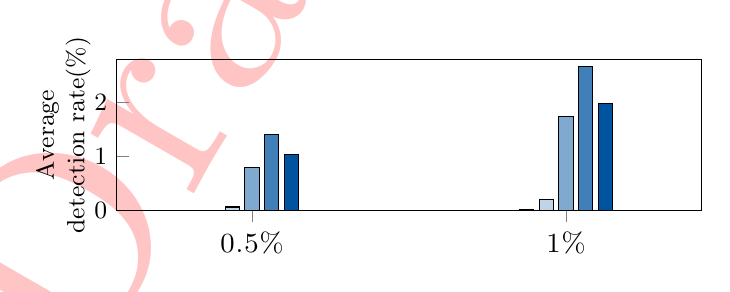
\begin{tikzpicture}[scale=1]
    \begin{axis}[
        ybar,
        enlargelimits=false, 
        scaled y ticks = false,
        %legend style={at={(0.02,0.74)},
        %anchor=west},
        legend style={at={(0.495,1.3)}, anchor=north,legend columns=-1, font=\footnotesize},
        bar width=0.18cm,
        width=9cm,
        height=3.5cm,
        style={align=center}, ylabel=Average\\detection rate(\%),
        ymax=2.800,
        ymin=-0.0,
        enlarge x limits=0.43,
        symbolic x coords={\textsc{0.5\%},\textsc{1\%}},
        xtick=data,
        ylabel near ticks,
        ylabel shift={-0.55em},
        xtick pos=left,
        ytick pos=left,
        legend image post style={scale=0.6},
        y tick label style={font=\small},
        y label style={font=\small}
    ]
    \addplot[fill=white] coordinates {(\textsc{0.5\%},0.0078125) (\textsc{1\%},0.0140625)};
    \addplot[fill=rwth_blue!25] coordinates {(\textsc{0.5\%},0.06607143) (\textsc{1\%},0.2125)};
    \addplot[fill=rwth_blue!50] coordinates {(\textsc{0.5\%},0.80390625) (\textsc{1\%},1.741015625)};
    \addplot[fill=rwth_blue!75] coordinates {(\textsc{0.5\%},1.409375) (\textsc{1\%},2.66875)};
    \addplot[fill=rwth_blue] coordinates {(\textsc{0.5\%},1.03203125) (\textsc{1\%},1.98671875)};

   % \legend{AES, DES, GOST, KECCAK, XTEA}
    \end{axis}
    \end{tikzpicture}  
    \vspace{-0.2cm}
    \caption{\label{fig:aver_dmux_set_all}\textsc{Set-All} average for D-MUX\vspace{0.25cm}}
\end{subfigure}
\begin{subfigure}{0.49\textwidth}
\centering
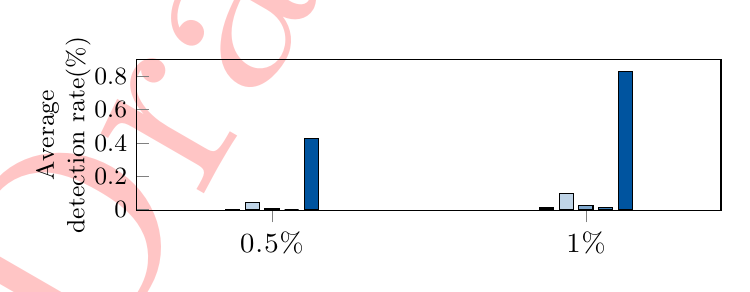
\begin{tikzpicture}[scale=1]
    \begin{axis}[
        ybar,
        enlargelimits=false, 
        scaled y ticks = false,
        %legend style={at={(0.02,0.74)},
        %anchor=west},
        legend style={at={(0.495,1.3)}, anchor=north,legend columns=-1, font=\footnotesize},
        bar width=0.18cm,
        width=9cm,
        height=3.5cm,
        style={align=center}, ylabel=Average\\detection rate(\%),
        ymax=0.9,
        ymin=-0.0050,
        enlarge x limits=0.43,
        symbolic x coords={\textsc{0.5\%},\textsc{1\%}},
        xtick=data,
        ylabel near ticks,
        ylabel shift={-0.55em},
        xtick pos=left,
        ytick pos=left,
        legend image post style={scale=0.6},
        y tick label style={font=\small},
        y label style={font=\small}
    ]
    \addplot[fill=white] coordinates {(\textsc{0.5\%},0.00078125) (\textsc{1\%},0.01074129)};
    \addplot[fill=rwth_blue!25] coordinates {(\textsc{0.5\%},0.04285714) (\textsc{1\%},0.1)};
    \addplot[fill=rwth_blue!50] coordinates {(\textsc{0.5\%},0.00976563) (\textsc{1\%},0.02539063)};
    \addplot[fill=rwth_blue!75] coordinates {(\textsc{0.5\%},0.0) (\textsc{1\%},0.0125)};
    \addplot[fill=rwth_blue] coordinates {(\textsc{0.5\%},0.42578125) (\textsc{1\%},0.82890625)};

   % \legend{AES, DES, GOST, KECCAK, XTEA}
    \end{axis}
    \end{tikzpicture}  
        \vspace{-0.2cm}

    \caption{\label{fig:aver_dmux_set_ll}\textsc{Set-Ll-Key} average for D-MUX\vspace{0.25cm}}
\end{subfigure}
%\end{figure*}
%%%%%%%%%%%%%%%%%%%%%%%%%%%%%%%%%%%%%%%%%


%%%%%%%% AVERAGE DETECTION FOR EPIC WITH DIFFERENT KEY SIZES OVER BENCHMARKS! %%%%%%%
%\begin{figure*}
\begin{subfigure}{0.49\textwidth}
\centering
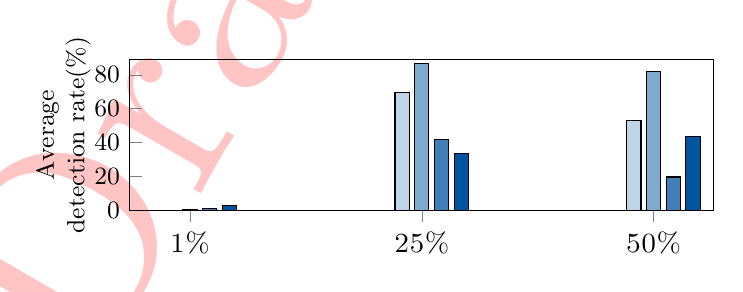
\begin{tikzpicture}[scale=1]
    \begin{axis}[
        ybar,
        enlargelimits=false, 
        scaled y ticks = false,
        %legend style={at={(0.02,0.74)},
        %anchor=west},
        legend style={at={(0.495,1.3)}, anchor=north,legend columns=-1, font=\footnotesize},
        bar width=0.18cm,
        width=9cm,
        height=3.5cm,
        style={align=center}, ylabel=Average\\detection rate(\%),
        ymax=89.000,
        ymin=-0.050,
        enlarge x limits=0.13,
        symbolic x coords={\textsc{1\%},\textsc{25\%}, \textsc{50\%}},
        xtick=data,
        ylabel near ticks,
        ylabel shift={-0.55em},
        xtick pos=left,
        ytick pos=left,
        legend image post style={scale=0.6},
        y tick label style={font=\small},
        y label style={font=\small}
    ]
    \addplot[fill=white] coordinates {(\textsc{1\%},0.0) (\textsc{25\%},0) (\textsc{50\%},0.0)};
    \addplot[fill=rwth_blue!25] coordinates {(\textsc{1\%},0.0) (\textsc{25\%},69.67) (\textsc{50\%},52.94)};
    \addplot[fill=rwth_blue!50] coordinates {(\textsc{1\%},0.4257) (\textsc{25\%},86.57) (\textsc{50\%},81.74)};
    \addplot[fill=rwth_blue!75] coordinates {(\textsc{1\%},1.084) (\textsc{25\%},42.08) (\textsc{50\%},19.75)};
    \addplot[fill=rwth_blue] coordinates {(\textsc{1\%},2.70) (\textsc{25\%},33.75) (\textsc{50\%},43.74)};

   % \legend{AES, DES, GOST, KECCAK, XTEA}
    \end{axis}
    \end{tikzpicture}  
       \vspace{-0.2cm}
 
    \caption{\label{fig:aver_epic_set_all}\textsc{Set-All} Average for EPIC\vspace{0.25cm}}
\end{subfigure}
\begin{subfigure}{0.49\textwidth}
\centering
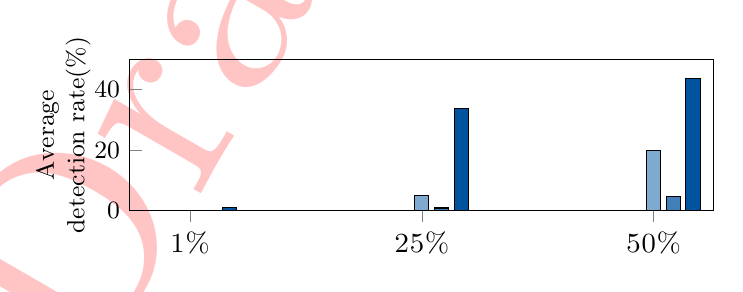
\begin{tikzpicture}[scale=1]
    \begin{axis}[
        ybar,
        enlargelimits=false, 
        scaled y ticks = false,
        %legend style={at={(0.02,0.74)},
        %anchor=west},
        legend style={at={(0.495,1.3)}, anchor=north,legend columns=-1, font=\footnotesize},
        bar width=0.18cm,
        width=9cm,
        height=3.5cm,
        style={align=center}, ylabel=Average\\detection rate(\%),
        ymax=50.00,
        ymin=-0.050,
        enlarge x limits=0.13,
        symbolic x coords={\textsc{1\%},\textsc{25\%}, \textsc{50\%}},
        xtick=data,
        ylabel near ticks,
        ylabel shift={-0.55em},
        xtick pos=left,
        ytick pos=left,
        legend image post style={scale=0.6},
        y tick label style={font=\small},
        y label style={font=\small}
    ]
    \addplot[fill=white] coordinates {(\textsc{1\%},0.0) (\textsc{25\%},0.0) (\textsc{50\%},0.0)};
    \addplot[fill=rwth_blue!25] coordinates {(\textsc{1\%},0.0) (\textsc{25\%},0.0) (\textsc{50\%},0.0)};
    \addplot[fill=rwth_blue!50] coordinates {(\textsc{1\%},0.0) (\textsc{25\%},4.833) (\textsc{50\%},20.0)};
    \addplot[fill=rwth_blue!75] coordinates {(\textsc{1\%},0.0) (\textsc{25\%},0.80) (\textsc{50\%},4.49)};
    \addplot[fill=rwth_blue] coordinates {(\textsc{1\%},0.9625) (\textsc{25\%},33.79) (\textsc{50\%},43.86)};

   % \legend{AES, DES, GOST, KECCAK, XTEA}
    \end{axis}
    \end{tikzpicture}  
        \vspace{-0.2cm}

    \caption{\label{fig:aver_epic_set_ll}\textsc{Set-LL-Key} Average for EPIC\vspace{0.25cm}}
\end{subfigure}
%\end{figure*}
%%%%%%%%%%%%%%%%%%%%%%%%%%%%%%%%%%%%%%%%%


%%%%%%%% AVERAGE DETECTION FOR ASSURE WITH DIFFERENT KEY SIZES OVER BENCHMARKS! %%%%%%%
%\begin{figure*}
\begin{subfigure}{\textwidth}
\centering
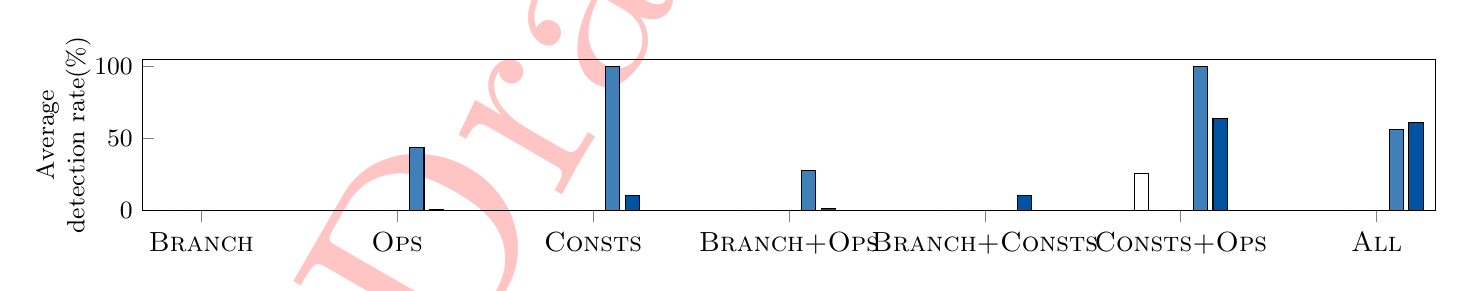
\begin{tikzpicture}[scale=1]
    \begin{axis}[
        ybar,
        enlargelimits=false, 
        scaled y ticks = false,
        %legend style={at={(0.02,0.74)},
        %anchor=west},
        legend style={at={(0.495,1.3)}, anchor=north,legend columns=-1},
        bar width=0.18cm,
        width=18cm,
        height=3.5cm,
        style={align=center}, ylabel=Average\\detection rate(\%),
        ymax=105.000,
        ymin=-0.050,
        enlarge x limits=0.05,
        symbolic x coords={\textsc{Branch},\textsc{Ops}, \textsc{Consts}, \textsc{Branch+Ops}, \textsc{Branch+Consts}, \textsc{Consts+Ops}, \textsc{All}},
        xtick=data,
        ylabel near ticks,
        ylabel shift={-0.55em},
        xtick pos=left,
        ytick pos=left,
        legend image post style={scale=0.9},
        y tick label style={font=\small},
        y label style={font=\small}
    ]
    \addplot[fill=white] coordinates {(\textsc{Branch},0.0) (\textsc{Ops},0) (\textsc{Consts},0.0) (\textsc{Branch+Ops},0.0) (\textsc{Branch+Consts},0.0) (\textsc{Consts+Ops},25.5625) (\textsc{All},0.0)};
    \addplot[fill=rwth_blue!25] coordinates {(\textsc{Branch},0.0) (\textsc{Ops},0) (\textsc{Consts},0.0) (\textsc{Branch+Ops},0.0) (\textsc{Branch+Consts},0.0) (\textsc{Consts+Ops},0.0) (\textsc{All},0.0)};
    \addplot[fill=rwth_blue!50] coordinates {(\textsc{Branch},0.0) (\textsc{Ops},0) (\textsc{Consts},0.0) (\textsc{Branch+Ops},0.0) (\textsc{Branch+Consts},0.0) (\textsc{Consts+Ops},0.0) (\textsc{All},0.0)};
    \addplot[fill=rwth_blue!75] coordinates {(\textsc{Branch},0.0) (\textsc{Ops},43.75) (\textsc{Consts},100.0) (\textsc{Branch+Ops},28.125) (\textsc{Branch+Consts},0.0) (\textsc{Consts+Ops},100.0) (\textsc{All},56.25)};
    \addplot[fill=rwth_blue] coordinates {(\textsc{Branch},0.0) (\textsc{Ops},0.78125) (\textsc{Consts},10.15) (\textsc{Branch+Ops},1.5625) (\textsc{Branch+Consts},10.15) (\textsc{Consts+Ops},64.06) (\textsc{All},60.94)};

   % \legend{AES, DES, GOST, KECCAK, XTEA}
    \end{axis}
    \end{tikzpicture}  
    
    \caption{\label{fig:aver_assure_set_all}\textsc{Set-All} Average for ASSURE. No detection for \textsc{Set-Ll-Key}}
\end{subfigure}
\caption{\label{fig:average_detections} Relative average detection rate for all 3 LL algorithms, for multiple key sizes and 5 benchmarks. \vspace{-0.4cm}}
\end{figure*}
Moreover, the examination of Fig.s~\ref{fig:hist_bitwise_dmux_1_set_all} and \ref{fig:hist_bitwise_dmux_1_set_ll} demonstrates that D-MUX is more prone to leak the later bits of the XTEA encryption key. However, EPIC indicates that the first bits of a 32-bit segment in the 128-bit secret are more susceptible to the XOR-XNOR locking scheme. Comparing Fig.~\ref{fig:hist_bitwise_dmux_1_set_all} with Fig.~\ref{fig:hist_bitwise_dmux_1_set_ll} shows that the number of leakages is diminished for the \textsc{Set-Ll-Key} attack scenario relative to the \textsc{Set-All}, as expected. A higher number of inputs that can be modified to leak information leads to a greater success rate. 
%In the case of benchmarks locked with EPIC, no difference between the two attack scenarios can be observed. The vast number of logic-locking key gates that can alter the information flow in the system does not necessitate the additional liberty of altering the other input bits, as provided by the \textsc{Set-All} attack.

Overall, each secret key bit can be forwarded to the output of the design with a probability of at least 20\% for the EPIC algorithm (25\% relative key size). However, this does not imply that all bits are vulnerable in the same benchmark of the set. For the smaller key sizes of the D-MUX algorithm, leakages in roughly 5\% of all benchmarks can be achieved for the later bits.
The following evaluation only focuses on the detections (DT) indicating a leakage. The AU and ND tests are both labeled as non-leakages. 


\subsection{Average Detection Rate Analysis}
The resulting average detection rates for all benchmarks are depicted in Fig.~\ref{fig:average_detections}.
%%%%%%%% AVERAGE DETECTION FOR MUX WITH DIFFERENT KEY SIZES OVER BENCHMARKS! %%%%%%%
%%%%%%%%%%%%%%%%%%%%%%%%%%%%%%%%%%%%%%%%%
For the graphs, the number of average detections in the set is divided by the length of the secret, allowing a comparison between the benchmarks. The effect of LL varies with the benchmark.% While the XTEA benchmark implements the highest relative number for D-MUX in the \textsc{Set-Ll-Key} scenario, fewer detections occur for the \textsc{Set-All} attack scenario. For the \textsc{Set-All} D-MUX case, KECCAK offers the most attack vectors. 

High average detection rates can be observed for the EPIC algorithm (see Fig.~\ref{fig:aver_epic_set_all} and Fig.~\ref{fig:aver_epic_set_ll}), which can use a bigger relative key size. Area-optimized designs like the XTEA and GOST benchmark are impacted significantly by the EPIC algorithm. The designs utilize FSMs that control the computation before releasing the ciphertext to the output. When XOR or XNOR gates are placed by EPIC in this control engine, the key gates can be used to flip bits and misuse some of the computational steps to allow a leakage of the data before it has been obfuscated sufficiently. 
%There is no discernible impact of EPIC LL on the confidentiality of the encryption key in the AES benchmark. Across all key lengths and attack scenarios, no encryption key bit has been found to be leaked as a result of LL. The absence of an FSM in the benchmark, which instead relies on pipelined computation, results in reduced susceptibility to control-related errors resulting from bit flips. This benefit is also observed in the DES benchmark, where the number of vulnerabilities is relatively low. 
Although the average detection rate seems to be reduced for the higher relative key size of 50\% compared to the 25\% one (see Fig.~\ref{fig:aver_epic_set_all}), it does not mean that fewer vulnerabilities are present in the benchmarks with more key gates. As explained before, the ND bits are not elaborated here. The ND tests require a longer runtime to decide whether the bits can be leaked (DT) or cannot be forwarded to the outputs of the design (S). The averages reflect the number of leakages that are at least present in the logic-locked benchmarks.
\begin{figure*}
% \begin{subfigure}{0.49\textwidth}
% \centering
% \begin{tikzpicture}[scale=1]
%     \begin{axis}[
%         ybar,
%         enlargelimits=false, 
%         scaled y ticks = false,
%         %legend style={at={(0.02,0.74)},
%         %anchor=west},
%         bar width=0.055cm,
%         width=9.2cm,
%         height=4cm,
%         style={align=center}, ylabel=Number of benchmarks,
%         xlabel = Number of bits leaked in a design,
%         ymax=650,
%         ymin=-0.050,
%         enlarge x limits=0.02,
%         xtick={0,16,32,48,64,80,96,112,128},
%         ylabel near ticks,
%         ylabel shift={-0.55em},
%         %xtick pos=left,
%         ytick pos=left,
%         y tick label style={font=\small},
%         y label style={font=\small},
%                         % now add the "horizontal line" ...
%         extra x ticks={0,40},
%         % ... don't show any label and ...
%         extra x tick labels={},
%         % ... adapt the style to your needs
%         extra x tick style={
%             % in case you should remove the grid from the "normal" ticks ...
%             xmajorgrids=true,
%             % ... but don't show an extra tick (line)
%             xtick style={
%                 /pgfplots/major tick length=0pt,
%             },
%             grid style={
%                 red,
%                 % to draw this line before the bars, move it a higher layer
%                 /pgfplots/on layer=axis foreground,
%             },
%             }
%     ]
%     \addplot[fill=rwth_blue!75, draw=none,] table {data/ATPG_mux_05_XTEA_timeout_10_sec_set_all_distr.txt};


%     %\legend{AES, DES, GOST, KECCAK, XTEA}
%     \end{axis}
%     \end{tikzpicture}  
%         \vspace{-0.55cm}
%     \caption{\label{fig:histogram_dmux_05_set_all}\textsc{Set-All} histogram for D-MUX 0.5\%}
% \end{subfigure}
% \begin{subfigure}{0.49\textwidth}
% \centering
% \begin{tikzpicture}[scale=1]
%     \begin{axis}[
%         ybar,
%         enlargelimits=false, 
%         scaled y ticks = false,
%         %legend style={at={(0.02,0.74)},
%         %anchor=west},
%         bar width=0.055cm,
%         width=9.2cm,
%         height=4cm,
%         style={align=center}, ylabel=Number of benchmarks,
%         xlabel = Number of bits leaked in a design,
%         ymax=650,
%         ymin=-0.050,
%         enlarge x limits=0.02,
%         xtick={0,16,32,48,64,80,96,112,128},
%         ylabel near ticks,
%         ylabel shift={-0.55em},
%         %xtick pos=left,
%         ytick pos=left,
%         y tick label style={font=\small},
%         y label style={font=\small},
%                         % now add the "horizontal line" ...
%         extra x ticks={0,32},
%         % ... don't show any label and ...
%         extra x tick labels={},
%         % ... adapt the style to your needs
%         extra x tick style={
%             % in case you should remove the grid from the "normal" ticks ...
%             xmajorgrids=true,
%             % ... but don't show an extra tick (line)
%             xtick style={
%                 /pgfplots/major tick length=0pt,
%             },
%             grid style={
%                 red,
%                 % to draw this line before the bars, move it a higher layer
%                 /pgfplots/on layer=axis foreground,
%             },
%             }
%     ]
%     \addplot[fill=rwth_blue!75, draw=none,] table {data/APTG_mux_05_XTEA_timeout_10_sec_set_ll_distr.txt};

%     %\legend{AES, DES, GOST, KECCAK, XTEA}
%     \end{axis}
%     \end{tikzpicture}  
%         \vspace{-0.55cm}
%     \caption{\label{fig:histogram_dmux_05_set_ll}\textsc{Set-Ll-Key} histogram for D-MUX 0.5\%}
% \end{subfigure}
%\end{figure*}
%%%%%%%%%%%%%%%%%%%%%%%%%%%%%%%%%%%%%%%%%


%%%%%%%% AVERAGE DETECTION FOR EPIC WITH DIFFERENT KEY SIZES OVER BENCHMARKS! %%%%%%%
%\begin{figure*}
\begin{subfigure}{0.49\textwidth}
\centering
\begin{tikzpicture}[scale=1]
    \begin{axis}[
        ybar,
        enlargelimits=false, 
        scaled y ticks = false,
        %legend style={at={(0.02,0.74)},
        %anchor=west},
        bar width=0.055cm,
        width=9.2cm,
        height=3.5cm,
        style={align=center}, ylabel=\# of benchmarks,
        xlabel = Number of bits leaked in a design,
        ymax=300,
        ymin=-0.050,
        enlarge x limits=0.02,
        xtick={0,16,32,48,64,80,96,112,128},
        ylabel near ticks,
        ylabel shift={-0.55em},
        %xtick pos=left,
        ytick pos=left,
        y tick label style={font=\small},
        y label style={font=\small, xshift=-0.5em},
                        % now add the "horizontal line" ...
        extra x ticks={0,46},
        % ... don't show any label and ...
        extra x tick labels={},
        % ... adapt the style to your needs
        extra x tick style={
            % in case you should remove the grid from the "normal" ticks ...
            xmajorgrids=true,
            % ... but don't show an extra tick (line)
            xtick style={
                /pgfplots/major tick length=0pt,
            },
            grid style={
                red,
                % to draw this line before the bars, move it a higher layer
                /pgfplots/on layer=axis foreground,
            },
            }
    ]
    \addplot[fill=rwth_blue!75, draw=none,] table {data/ATPG_mux_1_XTEA_timeout_10_sec_set_all_distr.txt};

    %\legend{AES, DES, GOST, KECCAK, XTEA}
    \end{axis}
    \end{tikzpicture}  
        \vspace{-0.55cm}
    \caption{\label{fig:histogram_dmux_1_set_all}\textsc{Set\_All} histogram for D-MUX 1\%}
\end{subfigure}
\begin{subfigure}{0.49\textwidth}
\centering
\begin{tikzpicture}[scale=1]
    \begin{axis}[
        ybar,
        enlargelimits=false, 
        scaled y ticks = false,
        %legend style={at={(0.02,0.74)},
        %anchor=west},
        bar width=0.055cm,
        width=9.2cm,
        height=3.5cm,
        style={align=center}, ylabel=\# of benchmarks,
        xlabel = Number of bits leaked in a design,
        ymax=450,
        ymin=-0.050,
        enlarge x limits=0.02,
        xtick={0,16,32,48,64,80,96,112,128},
        ylabel near ticks,
        ylabel shift={-0.55em},
        %xtick pos=left,
        ytick pos=left,
        y tick label style={font=\small},
        y label style={font=\small, xshift=-0.5em},
                        % now add the "horizontal line" ...
        extra x ticks={0,24},
        % ... don't show any label and ...
        extra x tick labels={},
        % ... adapt the style to your needs
        extra x tick style={
            % in case you should remove the grid from the "normal" ticks ...
            xmajorgrids=true,
            % ... but don't show an extra tick (line)
            xtick style={
                /pgfplots/major tick length=0pt,
            },
            grid style={
                red,
                % to draw this line before the bars, move it a higher layer
                /pgfplots/on layer=axis foreground,
            },
            }
    ]
    \addplot[fill=rwth_blue!75, draw=none,] table {data/ATPG_mux_1_XTEA_timeout_10_sec_set_ll_distr.txt};

    \end{axis}
    \end{tikzpicture}  
        \vspace{-0.55cm}
    \caption{\label{fig:histogram_dmux_1_set_ll}\textsc{Set-Ll-Key} histogram for D-MUX 1\%}
\end{subfigure}
%\end{figure*}
%%%%%%%%%%%%%%%%%%%%%%%%%%%%%%%%%%%%%%%%%


%%%%%%%% AVERAGE DETECTION FOR ASSURE WITH DIFFERENT KEY SIZES OVER BENCHMARKS! %%%%%%%
%\begin{figure*}
% \begin{subfigure}{0.49\textwidth}
% \centering
% \begin{tikzpicture}[scale=1]
%     \begin{axis}[
%         ybar,
%         enlargelimits=false, 
%         scaled y ticks = false,
%         %legend style={at={(0.02,0.74)},
%         %anchor=west},
%         bar width=0.055cm,
%         width=9.2cm,
%         height=4cm,
%         style={align=center}, ylabel=Number of benchmarks,
%         xlabel = Number of bits leaked in a design,
%         ymax=800,
%         ymin=-0.050,
%         enlarge x limits=0.02,
%         xtick={0,16,32,48,64,80,96,112,128},
%         ylabel near ticks,
%         ylabel shift={-0.55em},
%         %xtick pos=left,
%         ytick pos=left,
%         y tick label style={font=\small},
%         y label style={font=\small},
%                         % now add the "horizontal line" ...
%         extra x ticks={0,110},
%         % ... don't show any label and ...
%         extra x tick labels={},
%         % ... adapt the style to your needs
%         extra x tick style={
%             % in case you should remove the grid from the "normal" ticks ...
%             xmajorgrids=true,
%             % ... but don't show an extra tick (line)
%             xtick style={
%                 /pgfplots/major tick length=0pt,
%             },
%             grid style={
%                 red,
%                 % to draw this line before the bars, move it a higher layer
%                 /pgfplots/on layer=axis foreground,
%             },
%             }
%     ]
%     \addplot[fill=rwth_blue!75, draw=none,] table {data/ATPG_xor-xnor_1_XTEA_timeout_10_sec_set_all_distr.txt};

%     %\legend{AES, DES, GOST, KECCAK, XTEA}
%     \end{axis}
%     \end{tikzpicture}  
%         \vspace{-0.55cm}
%     \caption{\label{fig:histogram_epic_1_set_all}\textsc{Set\_All} histogram for EPIC 1\%}
% \end{subfigure}
% \begin{subfigure}{0.49\textwidth}
% \centering
% \begin{tikzpicture}[scale=1]
%     \begin{axis}[
%         ybar,
%         enlargelimits=false, 
%         scaled y ticks = false,
%         %legend style={at={(0.02,0.74)},
%         %anchor=west},
%         bar width=0.055cm,
%         width=9.2cm,
%         height=4cm,
%         style={align=center}, ylabel=Number of benchmarks,
%         xlabel = Number of bits leaked in a design,
%         ymax=999,
%         ymin=-0.050,
%         enlarge x limits=0.02,
%         xtick={0,16,32,48,64,80,96,112,128},
%         ylabel near ticks,
%         ylabel shift={-0.55em},
%         %xtick pos=left,
%         ytick pos=left,
%         y tick label style={font=\small},
%         y label style={font=\small},
%                         % now add the "horizontal line" ...
%         extra x ticks={0,67},
%         % ... don't show any label and ...
%         extra x tick labels={},
%         % ... adapt the style to your needs
%         extra x tick style={
%             % in case you should remove the grid from the "normal" ticks ...
%             xmajorgrids=true,
%             % ... but don't show an extra tick (line)
%             xtick style={
%                 /pgfplots/major tick length=0pt,
%             },
%             grid style={
%                 red,
%                 % to draw this line before the bars, move it a higher layer
%                 /pgfplots/on layer=axis foreground,
%             },
%             }
%     ]
%     \addplot[fill=rwth_blue!75, draw=none,] table {data/ATPG_xor-xnor_1_XTEA_timeout_10_sec_set_ll_distr.txt};

%     \end{axis}
%     \end{tikzpicture}  
%         \vspace{-0.55cm}
%     \caption{\label{fig:histogram_epic_1_set_ll}\textsc{Set-Ll-Key} histogram for EPIC 1\%}
% \end{subfigure}


% \begin{subfigure}{0.49\textwidth}
% \centering
% \begin{tikzpicture}[scale=1]
%     \begin{axis}[
%         ybar,
%         enlargelimits=false, 
%         scaled y ticks = false,
%         %legend style={at={(0.02,0.74)},
%         %anchor=west},
%         bar width=0.055cm,
%         width=9.2cm,
%         height=4cm,
%         style={align=center}, ylabel=Number of benchmarks,
%         xlabel = Number of bits leaked in a design,
%         ymax=78,
%         ymin=-0.050,
%         enlarge x limits=0.02,
%         xtick={0,16,32,48,64,80,96,112,128},
%         ylabel near ticks,
%         ylabel shift={-0.55em},
%         %xtick pos=left,
%         ytick pos=left,
%         y tick label style={font=\small},
%         y label style={font=\small},
%                         % now add the "horizontal line" ...
%         extra x ticks={8,60},
%         % ... don't show any label and ...
%         extra x tick labels={},
%         % ... adapt the style to your needs
%         extra x tick style={
%             % in case you should remove the grid from the "normal" ticks ...
%             xmajorgrids=true,
%             % ... but don't show an extra tick (line)
%             xtick style={
%                 /pgfplots/major tick length=0pt,
%             },
%             grid style={
%                 red,
%                 % to draw this line before the bars, move it a higher layer
%                 /pgfplots/on layer=axis foreground,
%             },
%             }
%     ]
%     \addplot[fill=rwth_blue!75, draw=none] table {data/ATPG_xor-xnor_25_XTEA_timeout_12_sec_set_all_distr.txt};

%     %\legend{AES, DES, GOST, KECCAK, XTEA}
%     \end{axis}
%     \end{tikzpicture}  
%         \vspace{-0.25cm}
%     \caption{\label{fig:histogram_epic_25_set_all}\textsc{Set\_All} histogram for EPIC 25\%}
% \end{subfigure}
% \begin{subfigure}{0.49\textwidth}
% \centering
% \begin{tikzpicture}[scale=1]
%     \begin{axis}[
%         ybar,
%         enlargelimits=false, 
%         scaled y ticks = false,
%         %legend style={at={(0.02,0.74)},
%         %anchor=west},
%         bar width=0.055cm,
%         width=9.2cm,
%         height=4cm,
%         style={align=center}, ylabel=Number of benchmarks,
%         xlabel = Number of bits leaked in a design,
%         ymax=80,
%         ymin=-0.050,
%         enlarge x limits=0.02,
%         xtick={0,16,32,48,64,80,96,112,128},
%         ylabel near ticks,
%         ylabel shift={-0.55em},
%         %xtick pos=left,
%         ytick pos=left,
%         y tick label style={font=\small},
%         y label style={font=\small},
%                         % now add the "horizontal line" ...
%         extra x ticks={12,62},
%         % ... don't show any label and ...
%         extra x tick labels={},
%         % ... adapt the style to your needs
%         extra x tick style={
%             % in case you should remove the grid from the "normal" ticks ...
%             xmajorgrids=true,
%             % ... but don't show an extra tick (line)
%             xtick style={
%                 /pgfplots/major tick length=0pt,
%             },
%             grid style={
%                 red,
%                 % to draw this line before the bars, move it a higher layer
%                 /pgfplots/on layer=axis foreground,
%             },
%             }
%     ]
%     \addplot[fill=rwth_blue!75, draw=none] table {data/ATPG_xor-xnor_25_XTEA_timeout_12_sec_set_ll_distr.txt};

%     \end{axis}
%     \end{tikzpicture}  
%         \vspace{-0.25cm}
%     \caption{\label{fig:histogram_epic_25_set_ll}\textsc{Set-Ll-Key} histogram for EPIC 25\%}
% \end{subfigure}

\begin{subfigure}{0.49\textwidth}
\centering
\begin{tikzpicture}[scale=1]
    \begin{axis}[
        ybar,
        enlargelimits=false, 
        scaled y ticks = false,
        %legend style={at={(0.02,0.74)},
        %anchor=west},
        bar width=0.055cm,
        width=9.2cm,
        height=3.5cm,
        style={align=center}, ylabel=\# of benchmarks,
        xlabel = Number of bits leaked in a design,
        ymax=85,
        ymin=-0.050,
        enlarge x limits=0.02,
        xtick={0,16,32,48,64,80,96,112,128},
        ylabel near ticks,
        ylabel shift={-0.55em},
        %xtick pos=left,
        ytick pos=left,
        y tick label style={font=\small},
        y label style={font=\small, xshift=-0.5em},
                        % now add the "horizontal line" ...
        extra x ticks={23,75},
        % ... don't show any label and ...
        extra x tick labels={},
        % ... adapt the style to your needs
        extra x tick style={
            % in case you should remove the grid from the "normal" ticks ...
            xmajorgrids=true,
            % ... but don't show an extra tick (line)
            xtick style={
                /pgfplots/major tick length=0pt,
            },
            grid style={
                red,
                % to draw this line before the bars, move it a higher layer
                /pgfplots/on layer=axis foreground,
            },
            }
    ]
    \addplot[fill=rwth_blue!75, draw=none] table {data/ATPG_xor-xnor_50_XTEA_timeout_10_sec_set_all_distr.txt};

    %\legend{AES, DES, GOST, KECCAK, XTEA}
    \end{axis}
    \end{tikzpicture}  
        \vspace{-0.25cm}
    \caption{\label{fig:histogram_epic_50_set_all}\textsc{Set\_All} histogram for EPIC 50\%}
\end{subfigure}
\begin{subfigure}{0.49\textwidth}
\centering
\begin{tikzpicture}[scale=1]
    \begin{axis}[
        ybar,
        enlargelimits=false, 
        scaled y ticks = false,
        %legend style={at={(0.02,0.74)},
        %anchor=west},
        bar width=0.055cm,
        width=9.2cm,
        height=3.5cm,
        style={align=center}, ylabel=\# of benchmarks,
        xlabel = Number of bits leaked in a design,
        ymax=85,
        ymin=-0.050,
        enlarge x limits=0.02,
        xtick={0,16,32,48,64,80,96,112,128},
        ylabel near ticks,
        ylabel shift={-0.55em},
        %xtick pos=left,
        ytick pos=left,
        y tick label style={font=\small},
        y label style={font=\small, xshift=-0.5em},
                % now add the "horizontal line" ...
        extra x ticks={24,78},
        % ... don't show any label and ...
        extra x tick labels={},
        % ... adapt the style to your needs
        extra x tick style={
            % in case you should remove the grid from the "normal" ticks ...
            xmajorgrids=true,
            % ... but don't show an extra tick (line)
            xtick style={
                /pgfplots/major tick length=0pt,
            },
            grid style={
                red,
                % to draw this line before the bars, move it a higher layer
                /pgfplots/on layer=axis foreground,
            },
            }
    ]
    \addplot[fill=rwth_blue!75, draw=none] table {data/ATPG_xor-xnor_50_XTEA_timeout_12_sec_set_ll_distr.txt};

    \end{axis}
    \end{tikzpicture}  
        \vspace{-0.25cm}
    \caption{\label{fig:histogram_epic_50_set_ll}\textsc{Set-Ll-Key} histogram for EPIC 50\%}
\end{subfigure}
\caption{\label{fig:histogram} Histogram illustrating the distribution of the netlists over the number of leakages for the XTEA benchmark. The red lines indicate the netlist(s) with the lowest highest number of leakages for the combination of key size and locking scheme. }
\vspace{-0.3cm}
\end{figure*}
ASSURE shows the highest relative leakage in the KECCAK benchmark in most locking modes for the \textsc{Set-All} attack scenario, as illustrated in Fig.~\ref{fig:aver_assure_set_all}. Three of the five crypto benchmarks show significant leakages introduced by ASSURE (KECCAK, XTEA and AES), while DES and GOST remain secure. This shows the impact of the hardware design on the introduction of vulnerabilities using LL. %As the number of detections for the \textsc{Set-Ll-Key} scenario is mostly zero for ASSURE, no illustration is provided. The evaluation of the AES benchmark for the \textsc{consts+ops} mode showed leakages, where a malicious LL key can leak 35 out of 128 encryption key bits. This vulnerability has been discussed in the exemplary data leakages (see Fig.~\ref{fig:assure_leak_example}).
The average detection rate for the EPIC 1\% benchmarks is lower than 10\% for all cryptographic algorithms. However, only considering the average is not sufficient, and outliers must be considered for a comprehensive threat assessment. Therefore, a histogram analysis is conducted to illustrate the number of leakages in each logic-locked gate-level netlist.
\subsection{Histogram Analysis}
To provide a clearer understanding of the number of leakages in each logic-locked netlist, Fig.~\ref{fig:histogram} presents a histogram analysis of the XTEA benchmark, which enables a comprehensive comparison of the algorithms across all relative key sizes and attack scenarios. Regrettably, no set of netlists is available for the ASSURE implementation, so no histogram analysis could be conducted for it. 
%%%%%%%%%%%%%%%%%%%%%%%%%%%%%%%%% HISTOGRAM %%%%%%%%%%%%%%%%
%%%%%%%%  %%%%%%%
%%%%%%%%%%%%%%%%%%%%%%%%%%%%%%%%%%%%%%%%%
Despite the fact that the complete set yields an average lower than 10\%, a closer look at the distributions, depicted in Fig.~\ref{fig:histogram_dmux_1_set_all} and Fig.~\ref{fig:histogram_dmux_1_set_ll}, reveals that a significant portion of the encryption key can still be compromised even for a smaller number of relative key sizes. 
%Specifically, 52\% (\textsc{Set-Ll-Key}) and 86\% (\textsc{Set-All}) of the complete encryption key bit can be leaked, meaning that a malicious LL key can easily forward more than half of the encryption key to the output. 
\textit{While the average detection rate provides an initial assessment of the security risk posed by LL schemes, it is worth noting that outliers highlight the true extent of their impact on the confidentiality property of an IC, which can be catastrophic.}
The evaluation of EPIC with higher relative key sizes finds that the minimum number of leakages exceeds 20 bits out of the 128-bit key. This implies that regardless of the key gates' placement in XTEA among the 1,000 benchmarks, modifying the LL key would leak at least 20 bits (Fig.~\ref{fig:histogram_epic_50_set_ll}).
%In all 4000 benchmarks, as shown in Fig.~\ref{fig:histogram_epic_25_set_all}-~\ref{fig:histogram_epic_50_set_ll}, the XTEA benchmark shows leakages. The center-mass of the histogram depicts the averages discussed earlier (Fig.~\ref{fig:average_detections}), without any significant outliers for higher relative key sizes, unlike EPIC 1\%. \textit{Although this vulnerability is unlikely, it still raises major security concerns while designing secure hardware.}

% \section{Discussion}


% All three LL algorithms have been shown to introduce security vulnerabilities into the hardware designs. The introduction of additional logic at random locations in secured hardware allows a misuse to leak information to an adversary.

% \subsection{MUX-Based Locking (D-MUX)}
% Introducing additional multiplexers to an already secured hardware design can lead to serious vulnerabilities by creating new signal paths for sensitive information. These paths allow a bypassing of the computational units responsible for obfuscating the signals. While the multiplexer can bypass any computational unit, the evaluation reveals that area-optimized designs are more susceptible to vulnerabilities compared to pipelined ICs such as the AES benchmark. Fig.~\ref{fig:dmux_leak_example} indicates that vulnerabilities were introduced in the AES benchmark, but higher leakages have been found in the XTEA and KECCAK benchmarks. The evaluation demonstrates that malicious LL keys can cause more than 25\% of an encryption key to be leaked after D-MUX introduces vulnerabilities into the cryptographic hardware accelerators. Additionally, D-MUX is the only LL algorithm that introduced vulnerabilities in all benchmarks for all attack scenarios. Note that these observations hold for all MUX-based locking algorithms, as the fundamental LL mechanism is the same across all schemes. 


% \subsection{XOR/XNOR-Based Locking (EPIC)}
% EPIC, a commonly used locking technique, has  certain weaknesses. While it does not introduce vulnerabilities that make it easy to bypass locking using multiplexers, the key gates' ability to flip bits poses a threat to data confidentiality. In area-optimized designs where FSMs control the flow, even minor bit flips can change states that can skip necessary computational steps, causing data leakage.
% Even for relatively small  key sizes of  1\%, the key gates can cause significant leakage of up to 86\% of the encryption key bits. While most benchmarks indicate a low number of vulnerabilities for this key size, outliers demonstrate the true danger that EPIC poses to area-optimized designs. The results indicate that the placement of key gates has a greater impact on the introduced security risks compared to the number of key gates. As the gates are randomly placed, the likelihood of selecting a vulnerable placement location is low, but it remains a significant security concern. The vulnerabilities can transfer to all XOR/XNOR-based locking policies.


% \subsection{RTL Locking (ASSURE)}
% ASSURE's impact on security properties is most notable in modes that involve constant locking. Since many cryptographic algorithms utilize lookup tables to apply non-linear functions to secrets, a large number of constants are replaced with LL keys, which can neutralize the function's effect on the secret and allow the unchanged secret to be forwarded. Additionally, the operations mode showed a significant impact for the KECCAK benchmark, with up to 44\% of the hashing input leaking under the \textsc{Set-All} attack scenario. Only AES showed vulnerabilities under \textsc{Set-Ll-Key}. However, it is still impractical to use the numerous LL key bits needed for obfuscation in ASSURE's constant mode. The AES benchmark necessitates 704,855 key bits to leak only 35 encryption key bits for the mentioned locking mode. Although no vulnerabilities were found for ASSURE when assessing the \textsc{Set-Ll-Key} scenario with the other benchmarks, it is essential to highlight the significant vulnerabilities in the \textsc{Set-All} scenario for ASSURE. The identified vulnerabilities offer important observations for the design of high-level LL policies---a promising new field of LL.


% \subsection{Comparison}
% All three LL schemes introduce vulnerabilities into cryptographic hardware accelerators. While some benchmarks showed minor information leakages for certain relative key sizes and algorithm combinations, EPIC and D-MUX exhibited outliers that significantly impacted the security of sensitive signals. D-MUX's multiplexers bypass security and cause leakage, while EPIC allows attacks on the control engine. In the evaluation, ASSURE showed the least amount of leakage for the \textsc{Set-Ll-Key} attack scheme but still introduced leakages for 100\% of the encryption key bits when obfuscating constants. \textit{Therefore, whether conducted at the RTL or gate level, LL can introduce major security risks to an IC.}

\subsection{Limitations and Future Work}
 As mentioned before, a relatively high number of ND tests are still present in the final results. The evaluation for removing the ND tests takes a significant amount of time. No feasible increase of the time limit for the ATPG framework resulted in the change of the tests' label. \textit{However, it means that the number of introduced leakages into the benchmark can be even higher than presented here.} Quantitative information flow analysis methods may identify additional vulnerabilities~\cite{qflow, qflow2}. These frameworks use probabilistic analysis to quantify the amount of information an adversary can gain about a secret by observing the outputs.
% While a SAT attack might offer an even higher attack surface, we decided to use an ATPG framework, which offered an analysis supported by a reliable commercial tool.

% Furthermore, ATPG analysis provides information only on leakages that allow the direct forwarding of sensitive data to the output port. Other vulnerabilities that could allow adversaries to better guess a secret are not evaluated. Quantitative information flow analysis methods, such as those employed in the QFlow framework, may identify additional vulnerabilities~\cite{qflow, qflow2}. These frameworks use probabilistic analysis to quantify the amount of information an adversary can gain about a secret by observing the outputs.

% To date, no analysis has been conducted on how to avoid the vulnerabilities introduced into the system by LL. Thus, further examination of this security risk is necessary. This examination could include possible mitigations for the security properties present in the original non-logic-locked benchmarks.
Possible mitigations include iterative approaches that analyze the security properties after LL the circuit are a possibility. If vulnerabilities are identified, the circuit would need to be logic-locked again. 
%Additionally, the LL schemes could be modified to forward security properties to the stage in the locking algorithm that decides on the placement of the modifications. As a result, the placement algorithm could focus on avoiding corruption of the security properties.

\section{Conclusion}

In this study, we investigated the impact of logic locking on the confidentiality of sensitive signals in hardware descriptions. \textit{Through path sensitization, we found that some cryptographic benchmarks, which were deemed secure before the application of logic locking, exhibited major data leakages after logic locking was applied}. While ASSURE is relatively secure against attacks that modify only the LL key, it can still leak up to 100\% of the key when all inputs are under the attacker's control. Compared to ASSURE, EPIC exhibits a significantly higher susceptibility to leakage, with up to 73.83\% of the encryption key being compromised solely by modifying the logic locking key. Furthermore, D-MUX leaks only up to 25\% of the encryption key in the same attack scenario. \textit{Therefore, it is evident that logic locking can pose a significant risk to the confidentiality of sensitive data in hardware designs.} %\textcolor{red}{}Having established the notable influence of logic locking on circuits with prior security measures, we project an even more substantial effect on less secured logic locked accelerators or processors, such as the MiG-V~\cite{mig_v}.
%We are the first to discover novel security vulnerabilities caused by logic locking. 
Nonetheless, we acknowledge logic locking's ability to protect the IC from hardware Trojans throughout the supply chain, albeit at the cost of compromising confidentiality.
%\textcolor{red}{}With the addition of obfuscation hardware, extra functionality may be introduced, compromising security properties such as confidentiality, if not designed carefully.
%To mitigate this risk, other security metrics must be considered when obfuscating the hardware, or an additional security check must be performed after the obfuscation to \textit{avoid jeopardizing} the proven security properties.



%-------------------------------------------------------------------------------
%\clearpage
%\balance
\bibliographystyle{IEEEtran}
\bibliography{bibtexentry}


%%%%%%%%%%%%%%%%%%%%%%%%%%%%%%%%%%%%%%%%%%%%%%%%%%%%%%%%%%%%%%%%%%%%%%%%%%%%%%%
\end{document}
%%%%%%%%%%%%%%%%%%%%%%%%%%%%%%%%%%%%%%%%%%%%%%%%%%%%%%%%%%%%%%%%%%%%%%%%%%%%%%%%

%%  LocalWords:  endnotes includegraphics fread ptr nobj noindent
%%  LocalWords:  pdflatex acks
